
The software maintenance task for web applications comes with the
extra burden of database  maintenance, including both data format changes, 
like adding
or deleting a table column, and data constraint changes, like
changing the length requirement of a password field.
In this section, we study how constraints evolve across versions
and the related data-maintenance challenges.

\paragraph{\bf How often do constraint-related changes occur?} 
% As shown in  Table~\ref{table:firstlatestcomparison}, 
We first checked the first commit of each application, and found {\it no}
data constraints in all but 3 applications (Ds, Lo, FF).
For all applications, the majority of the constraints were added in later commits.

%We then check how often data constraints change across versions. 
%Different applications release software versions at different frequency: Gitlab has 7 releases within a single month\shan{is this average speed?}, while xxx \shan{give a slow example}. 
As shown in Table~\ref{table:percentage}, 21--95\% (avg. 49\% across all apps) of code versions contain
 data constraints that are different from those 
 in its previous version, 
 indicating that constraint changes are common. Note that, for
 most applications, we treat one code release as one version; for
 4 applications that do not specify release/version information,
 we treat every 100 code commits as one version.
 
 \begin{table}
\centering
% \setlength{\tabcolsep}{1.5pt}  
\caption{App. versions with constraint changes (\#Version$_\text{C}$)}
\resizebox{0.6\columnwidth}{!}{
%\begin{tabular}{l@{\hspace{0.1in}}r@{\hspace{0.1in}}r@{\hspace{0.1in}}r@{\hspace{0.1in}}r@{\hspace{0.1in}}r@{\hspace{0.1in}}r@{\hspace{0.1in}}r@{\hspace{0.1in}}r@{\hspace{0.1in}}r@{\hspace{0.1in}}r@{\hspace{0.1in}}r@{\hspace{0.1in}}r@{\hspace{0.1in}}}
\begin{tabular}{lrrrrrrrrrrrr}
\toprule
& {\color[HTML]{FE0000} Ds} & {\color[HTML]{000000} Lo} & {\color[HTML]{FE0000} Gi} & {\color[HTML]{FE0000} Re} & {\color[HTML]{FE0000} Sp} & {\color[HTML]{FE0000} Ro} & {\color[HTML]{000000} Fu} & {\color[HTML]{FE0000} Tr} & {\color[HTML]{FE0000} Da} & {\color[HTML]{FE0000} On} & {\color[HTML]{000000} FF} & {\color[HTML]{000000} OS}  \\ \midrule
\#Version & 316 & 19 & 1040 & 159 & 253 & 31 & 7 & 26 & 39 & 86 & 12 & 95 \\ \midrule
\#Version$_\text{C}$ & 187 & 18 & 563  & 44  & 89  & 20 & 4 & 12 & 26 & 18 & 10 & 41 \\ \midrule
\%Version$_\text{C}$  & 59\% & 95\% & 54\% & 28\% & 35\% & 65\% & 57\% & 46\% & 67\% & 21\% & 83\% & 43\% \\ \bottomrule
\end{tabular}
}

\label{table:percentage}
\footnotesize{All types in Table \ref{table:constraintdeftax} except for custom sanity checks are considered.\\Red apps use a release as a version; Black apps use every 100 commits as a version.}
{\footnotesize }
\end{table}

 
\iffalse 
\begin{table}

\setlength{\tabcolsep}{2pt}  
\caption{\# Data constraints in the first and the latest version}
\resizebox{0.7\columnwidth}{!}{
\begin{tabular}{lrrrrrrrrrrrr}

\toprule
& Ds   & Lo  & Gi   & Re  & Sp  & Ro  & Fu & Tr  & Da  & On  & FF  & OS  \\
\midrule
first & 181 & 66 & 0 & 0 & 0 & 0 & 0 & 0 & 0 & 0 & 13 & 0\\
\midrule
latest  & 1764 & 160 & 1970 & 693 & 131 & 594 & 47 & 142 & 482 & 453 & 177 & 413 \\
\bottomrule
\end{tabular}
}
\label{table:firstlatestcomparison}
\footnotesize{All types in Table \ref{table:constraintdeftax} except for custom sanity checks are considered.}
\end{table}
\fi 

% \begin{table}[h]
% \caption{App. versions with constraint changes (\#Version$_\text{C}$)}
% \resizebox{\columnwidth}{!}{
% \begin{tabular}{l@{\hspace{0.1in}}r@{\hspace{0.1in}}r@{\hspace{0.1in}}r@{\hspace{0.1in}}r@{\hspace{0.1in}}r@{\hspace{0.1in}}r@{\hspace{0.1in}}r@{\hspace{0.1in}}r@{\hspace{0.1in}}r@{\hspace{0.1in}}r@{\hspace{0.1in}}r@{\hspace{0.1in}}r@{\hspace{0.1in}}}
% \toprule
% & Ds & Lo & Gi & Re & Sp & Ro & Fu & Tr & Da & On & FF & OS\\
% \midrule
% \#Version & 339 & 19 & 949 & 144 & 197 & 18 & 7 & 39 & 196 & 83 & 12 & 91 \\
% \midrule
% \#Version$_\text{C}$ & 177 & 15 & 173 & 65 & 66 & 15 & 4 & 19 & 77 & 11 & 11 & 27\\
% \midrule
% \%Version$_\text{C}$ & 52\% & 79\% & 18\% & 45\% & 34\% & 83\% & 57\% & 49\% & 37\% & 13\% & 92\% & 27\%
% \\
% \bottomrule
% \end{tabular}
% }
% \label{table:issueapp}

% {\footnotesize }
% \end{table}

% \junwen{the new table of release is saved at tables/percentageofchangedrelease.tex}

 \paragraph{\bf What triggered changes?}
We categorize all the cross-version changes about DB constraints
and application validation constraints into three types: 
(1) Add Column: adding constraints to a data column that did not exist in previous version;
(2) Add Constraint: 
adding constraints to an existing data column that was not associated
with that specific type of constraints, like adding a length
constraint to a data field that had no length constraint previously;
(3) Change Constraint: changing the detailed requirement of a constraint that already
existed in previous version.

% \shan{do these applications really no have public release versions?
% is it possible that the multiple versions here actually belong to the same
% public release?} \junwen{8 applications have release versions}


%Ideally, most constraint changes should belong to the Add-Column type, which would indicate stable and timely constraint maintenance. However, this is often not true ---
What is alarming from the result (Figure~\ref{fig:constraints-num})
is that the Add-Column type only 
contributes to around or lower than 50\% of changes in 
5 out of the % data source: https://docs.google.com/spreadsheets/d/1h8LZAczQoTkSXWalqBymrRVKCTxuxaH946snlQDnRwk/edit?usp=sharing 
12 applications. On the other hand, 13--67\% of constraint changes
(23\% across all applications) are adding new types of constraints to columns that already existed in earlier versions (i.e., tightening the constraints),
indicating that constraint addition is often developers' after-thoughts.
Changing existing constraints is much less common, but is still not rare, contributing to more than 10\% of constraint
changes in 4 applications.
% \shan{Junwen, pls change figure 2,
% so that its height is this short, but the in-figure caption is more readable?}
% Lobsters, gitlab, diaspora
 


\begin{figure} 
    \centering
    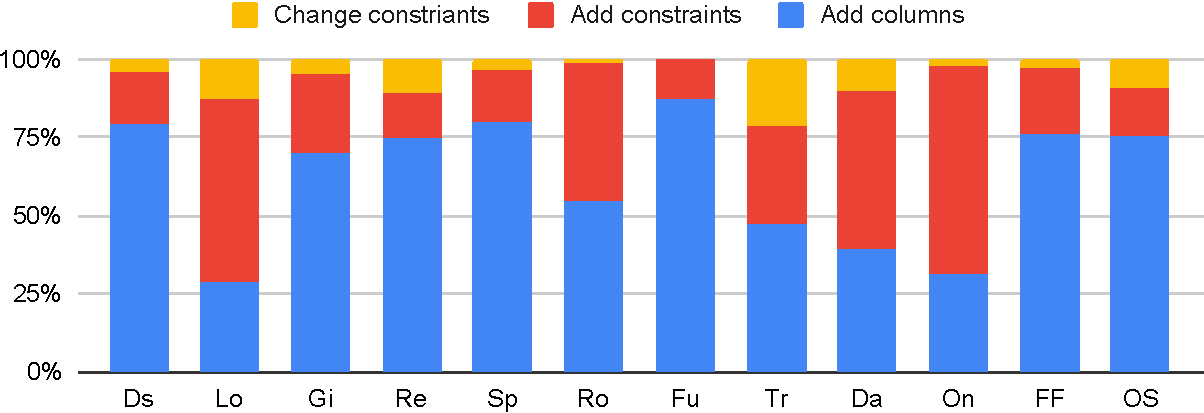
\includegraphics[width=0.6\columnwidth]{constraints//figs/breakdown-release.pdf}
    \caption{Breakdown of \# of adding/changing constraints 
\\   
%\junwen{the figure of release unit is saved as figs/breakdown-release.pdf}
}

    \label{fig:constraints-num}
\end{figure}


\paragraph{\bf Summary} It is problematic
that around or more than a quarter of constraint-related code changes in
most applications are about adding constraints to already existing data columns. This indicates a widely existing vulnerability that allows constraint-violating data to be stored into the database before the correct constraints are imposed. 
Tools are needed to help developers add 
suitable constraints whenever a new data column is created and 
warn of data that is incompatible with the newly added constraints.
  

% \begin{figure}[h]
%     \centering
%     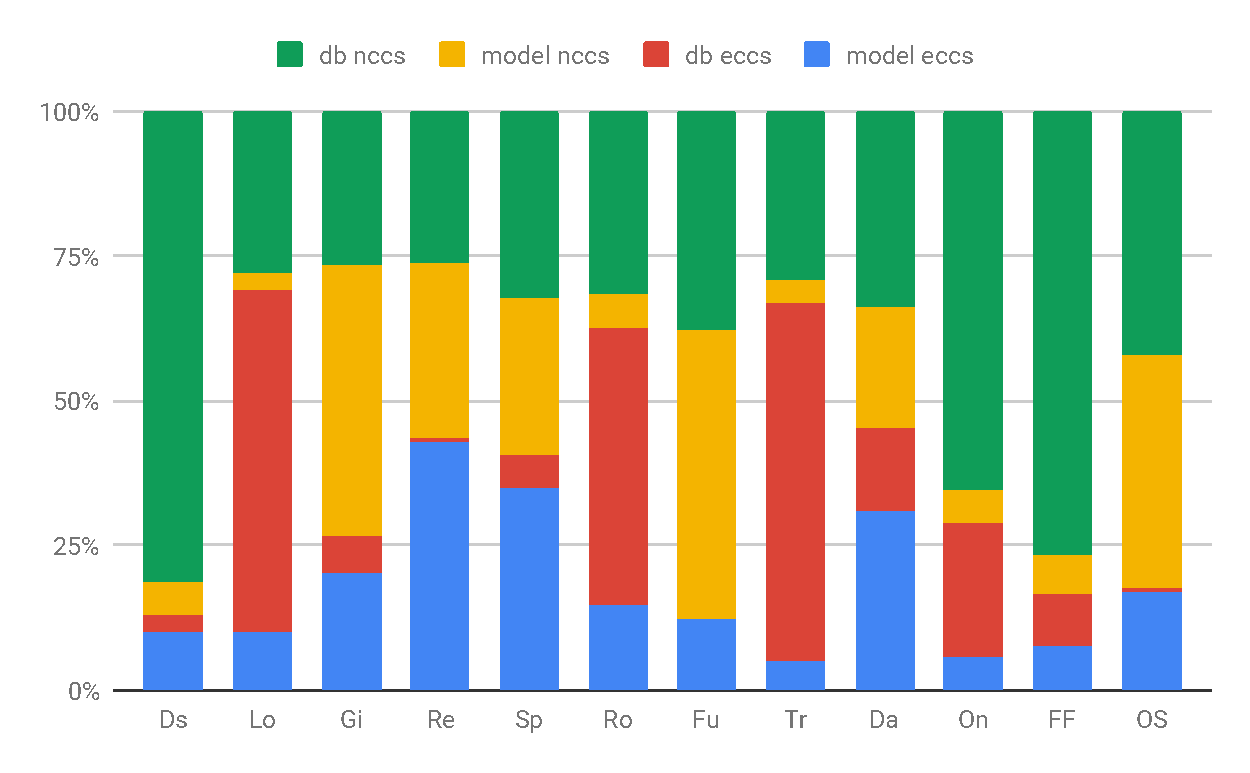
\includegraphics[width=\columnwidth]{figs/existing-new-columns.pdf}
%     \caption{Breakdown of \# of constraints on new/exsiting columns}
%     \footnotesize{nccs: adding constraints on new columns; 
%     eccs: 
%     adding constraints on existing columns}
%     \label{fig:exist-column}
% \end{figure}


% Later
% \begin{figure}[h]
%     \centering
%     \includegraphics[width=\columnwidth]{figs/total.pdf}
%     \caption{Trend of Changing/adding constraints towards line of code change\shan{???first, may want to draw the figures in a different way; second, if absolutely no trend, not worth the space}}
%     \label{fig:exist-column}
% \end{figure}